\chapter{Theoretical Background}
Since Turing wrote about the imitation game\cite{imitationgame} and Rosenblatt about the perceptron\cite{perceptron}, learning machines have stayed in the minds of computer scientists and science fiction writers. 
Improvements in computation and algorithms have since then taken Machine Learning(ML) past human level performance in multiple areas such as image recognition\cite{youtubecats}\cite{deepface}, board games like chess\cite{alphazero} or go\cite{alphago}, TV game-shows like Jeopardy\cite{jeopardy} or e-sports such as DOTA2\cite{dota2}.

\section{Machine Learning}
\label{background:ML}
 
In Machine Learning, the fields of statistics, mathematics, and data analysis are combined and applied to automatic modeling of data. Its three main sub-fields, supervised, unsupervised and Reinforcement Learning (RL) covers a vast number of structures and techniques. This thesis will focus on the flag-ship of Machine Learning, the Artificial Neural Network,  set it in a supervised learning scenario where it is applied to a classification problem.

\begin{figure}[ht] 
\centering
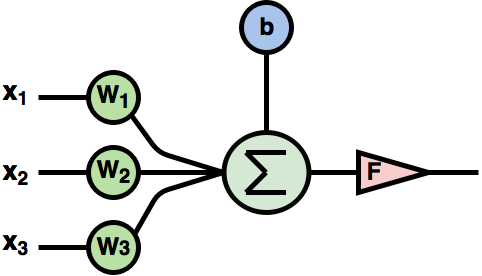
\includegraphics[width=0.7\linewidth]{Chapters/2.Background/figures/artificial_neuron.png}
\caption[Visualization of a artificial neuron]{Visualization of a artificial neuron with 3 inputs. Each input \(x_{i}\) is multiplied with a corresponding trainable weight \(W_{i}\) before the products are all summed together with a bias \(b\). The resulting value is then passed through a activation function \(F\)}
\label{fig:artificialneuron}
\end{figure}

Supervised learning is a way to teach some machine learning system patterns in annotated data. In a dataset \(\left [X, Y \right] \), each data-point \(x_{i}\) corresponds to a label or ground truth \(y_{i}\). In the context of an Artificial Neural Network, each \(x_{i}\) is fed through the network where the parameters are fitted against the target \(y_{i}\) using some optimization algorithm. 

Inspired by the structure of the brain, the ANN or \textit{Neural Network} (NN) consists of layers of artificial neurons like the one visualized in figure \ref{fig:artificialneuron}. Each neuron has a number \(n\) of inputs where each input is scaled by a tunable \textit{parameter} or \textit{weight} \(W_{i}\) and summed together including a bias \(b\) before it is passed through a activation function \(F\).

\begin{equation}
    F(\sum_{i=1}^{n}W_{i}x_{i} + b) = neuron output
\end{equation}

Two of the most commonly used activation functions are the rectified linear unit function (ReLU) and the softmax function, which is the generalization of binary logistic regression to multiple classes. ReLU merely evaluates to the maximum of neuron output and 0, which sets zero if the output is negative and keeps positive outputs. Softmax, on the other hand, approximates a probability by scaling the output of a set of neurons to have a sum between 0 and 1 and are used in classification where the output corresponds to the probability of each class being the correct label. These two activation functions will play a role in the later experiments (see sections \ref{exp1:implementation}, \ref{exp2:implementation}, and \ref{exp3:implementation}) in this thesis, where softmax will be used as the final activation layer to be the basis of classification. ReLU is used as activation function throughout the rest of the neural networks. 

These types of systems \textit{learn} to approximate a function based on the data provided to the network. Each data point \(x_{i}\) consist of multiple features (\(x_{ij}\)'s), which is fed through one or more layers of neurons that in the end output a prediction \(\hat{y}_{i}\). This prediction is then compared to the ground truth with a loss function\footnote{Also called cost function, error function or objective function} which calculates the difference between expected output \(y_{i}\) and observed output \(\hat{y}_{i}\).
For this thesis, the loss function used is \textit{cross-entropy} which is well suited for classification with softmax activation\cite{softmaxcrossentropy}.

The goal of the training is to minimize the loss function for a given dataset. To accomplish this, each calculated loss is backpropagated through the neural network, and an optimization algorithm is used to calculate the gradient of the weights with regards to the layer output and then to adjust the weights. The optimizers used in the experiments in chapter \ref{exp1}, \ref{exp2}, and \ref{exp3} are stochastic gradient descent(SGD)\cite{sgd} and Adaptive Moment Estimation (Adam)\cite{adam}. 

The function approximation properties of neural networks are used as a regression tool in data analysis, prediction, and reward signal estimation for RL among other areas, but is as mentioned, applied to classification in this thesis.

The final softmax layer outputs an estimated probability for each label given some input where the label given highest probability is selected as the model's prediction. As long as the input features to the network is correlated to the label in some way and there is enough training data, the neural network will adapt to the patterns in input features and learn one or more classification rules. In the case of an image classifier, the network is provided with the raw pixel values in the image. A normal, fully connected neural network\footnote{Also called affine, or dense networks.} is badly suited for this type of classification since attributes in images often change location or scale. E.g., a picture of a dog is still a picture of a dog if the image is rotated upside down, rescaled, or framed differently. To account for all these cases, the dataset used would have to contain multiple examples of all these variations.
\begin{figure}[ht] 
    \centering
    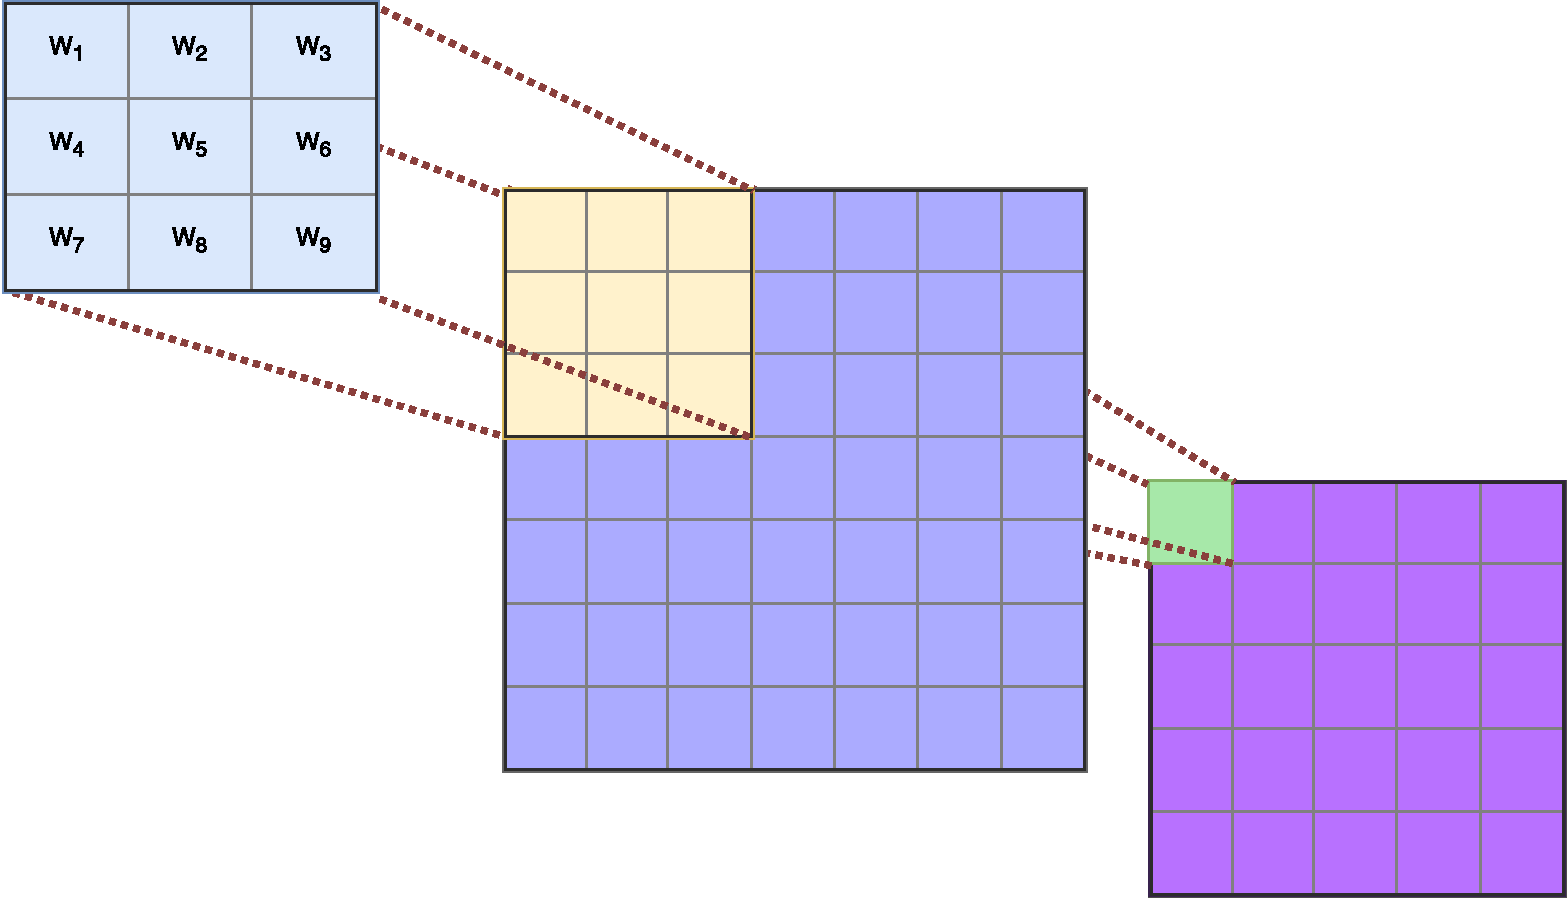
\includegraphics[width=\linewidth]{Chapters/2.Background/figures/convolution.pdf}
    \caption[Illustration of convolutional operation.]{Illustration of convolutional operation. The teal matrix(Kernel) contains convolutional parameters. These are element-wise multiplied by the overlapping (yellow) pixels in the image (blue matrix) and added together. The resulting value is placed in the corresponding location in the output feature map (purple). The convolutional operation is completed by sliding or \textit{striding} the yellow window across the original image.}
    \label{fig:conv}
\end{figure}
To remedy this, image classifiers usually contains convolutional layers which are invariant to scale, rotation or translation. In a convolutional layer, a \textit{kernel} of trainable weights are convolved with the input image. This results in what is called a \textit{feature map}, where the image size is reduced by some number of pixels\footnote{In cases where we want to keep the image dimension through the convolutions, the image can be padded first.} depending on the size of the kernel. However, while the outputs spatial dimensions are reduced, the number of channels in the image is usually increased. The intent of this is to raise the level of abstraction in the feature map for each convolutional layer. 

In a convolutional operation, a kernel is slid across an image, and for every overlap between the kernel and an image section, the kernel weights are multiplied with its corresponding pixel and summed (see figure \ref{fig:conv}). As with fully connected layers, the operations performed in each step is multiplication and summation, but here, each pixel in the output feature map contains some spatial information.The size of this spatial area covered by each feature can be controlled by the kernel size and how much the kernel is moved (called \textit{stride}) between each kernel multiplication.
Networks consisting of multiple layers of convolution is called Convolutional Neural Networks (CNNs)\footnote{These are the types of modules used in implementing the quinary MNIST classification in chapter \ref{exp1}, and in all modules in chapters \ref{exp2} and \ref{exp3}}.

\begin{figure}[ht] 
    \centering
    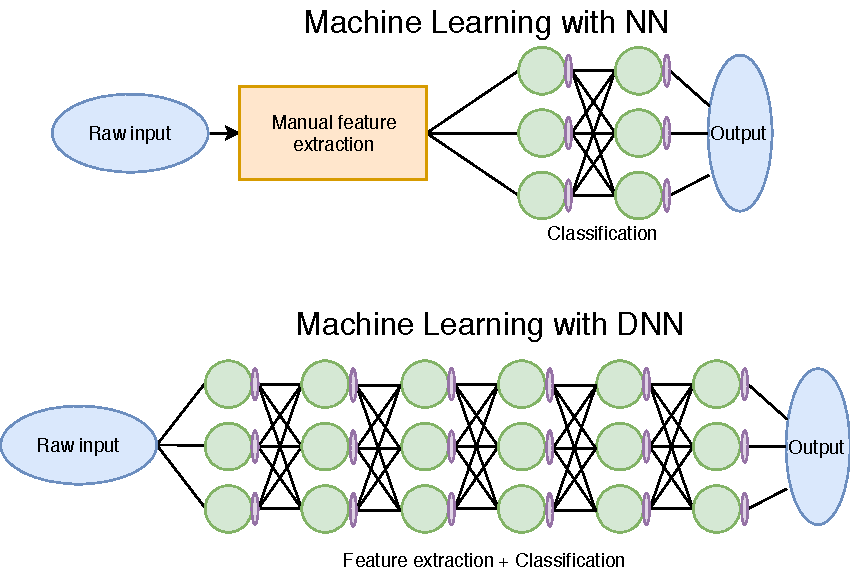
\includegraphics[width=\linewidth]{Chapters/2.Background/figures/NNvsDNN_NY.pdf}
    \caption[NN vs. DNN]{Figure visualizes the difference between traditional Neural Networks and Deep Neural Networks. Some feature extraction or preprocessing is performed on the raw input in the case of a NN, where the raw input is fed directly through the network in the case of Deep Learning. Each artificial neuron (\textit{green}) are fully connected in both cases, and each neurons output is passed through some activation (\textit{purple}).}
    \label{fig:NNvsDNN}
\end{figure}

\section{Deep Learning}
Usually, when talking about CNNs, the line is crossed into \textit{Deep Learning}. In each layer of convolution, the spatial size is reduced while the number of channels increases. This means the information processed shifts gradually from a spatially encoded "image" to an encoding in feature space, making a CNN capable of turning raw image input into a higher order feature representation. That is why deep Convolutional Neural Networks can be said to be performing feature extraction on its own.

\begin{figure}
    \begin{subfigure}[ht]{0.49\linewidth}
        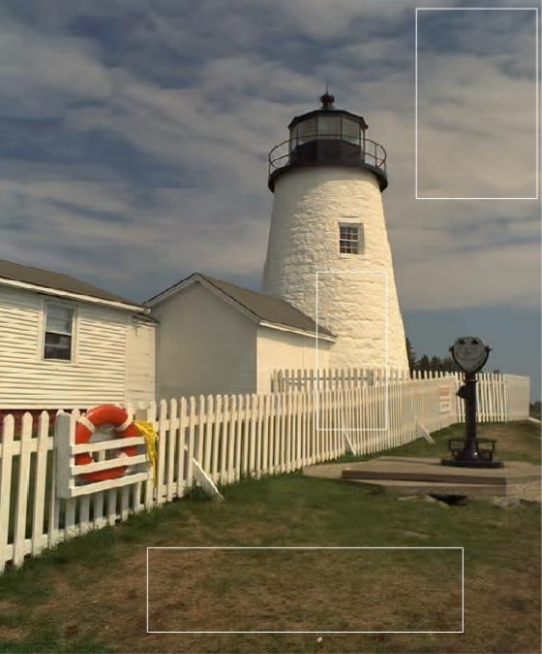
\includegraphics[width=\linewidth]{Chapters/2.Background/figures/original.png}
        \caption{Original image}
    \end{subfigure}
    \hfill
    \begin{subfigure}[ht]{0.49\linewidth}
        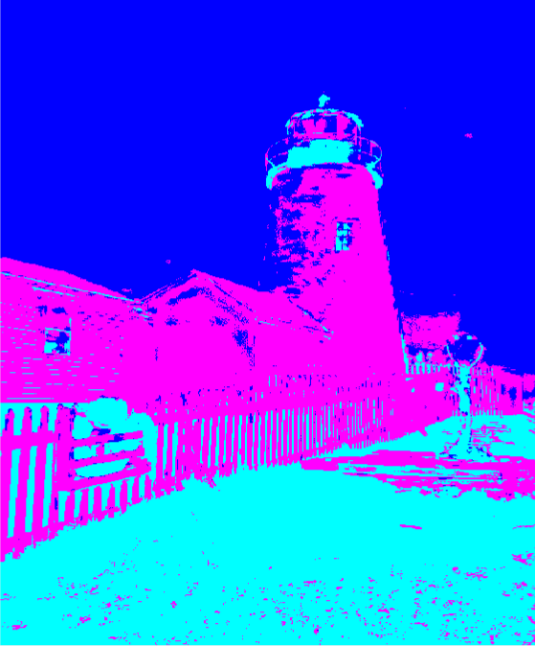
\includegraphics[width=\linewidth]{Chapters/2.Background/figures/segmentation.png}
        \caption{Segmented image}
    \end{subfigure}
    \caption[Image segmentation]{Example of image segmentation. Original image have been segmented into three classes: \textit{sky}(blue), \textit{ground}(teal) and \textit{building}(pink). The three boxes in the original image is pixels used as training data for each class.}
    \label{fig:semanticsegmentation}
\end{figure}

How deep a \textit{Deep Neural Network}(DNN) is made depends on the task at hand. Take for example a complicated task such as \textit{semantic segmentation}. Semantic segmentation is a variation of image classification where each pixel in an input image is assigned a class label, and the whole of the image is segmented into its semantic parts (see figure \ref{fig:semanticsegmentation}). In a CNN performing this task, the spacial information in the original image cannot be entirely removed since we want to create a new image with the original dimensionality and spatial locations of objects. Such a neural network would need to have enough \textit{capacity} to retain all needed knowledge to complete the task. The capacity of a NN is how much information can be stored in its weights, and is a measure highly correlated to the network's number of parameters. Managing capacity needs of a NN is part of the motivation behind encouraging module reuse in experiments 1, 2 and 3 (see chapters \ref{exp1}, \ref{exp2} and \ref{exp3}).

Intuitively, the difference between NNs and Deep neural networks (DNN) is just the number of layers in the model, but functionally we can view the DNN as a network performing its own feature extraction from raw data, like in the visualization in figure \ref{fig:NNvsDNN}. 

Complex Deep Learning models have been effective at such tasks as image classification\cite{imageclassification}, Natural Language Processing\cite{deepnlp} and Reinforcement Learning\cite{deepreinforcementlearning}. The architecture and use of each of these types of DNNs are dependent on the input type and problems they are applied to as well as resource limitations.

\subsection{Transfer Learning}
\label{background:TL}
The considerable number of trainable parameters in Deep Learning increase the data resources needed. If the amount of available labeled training data is restricted, one solution is to train on a similar task for which there is a significant amount of data and apply the patterns learned to the original task. It is shown that this reuse of knowledge as a basis for further learning can yield better results than what was possible with the original dataset\cite{pathnet, progressiveneuralnetworks, tradaboost}. Called \textit{Transfer Learning} (TL), this approach is to use generalized knowledge in one domain as a basis for future learning in another. With the goal of achieving more effective learning in the target domain or even reaching a lower convergence point for the loss, TL shares some common ground with the field of multi-task learning, where the same model is applied to multiple tasks. 

We can define transfer learning as trying to learn a target conditional probability distribution \(P(Y_{t}|X_{t})\) within a domain \(\mathcal{D}_{t}\), based on information gained from learning a source task \(\mathcal{T}_{s}\) in the source domain \(\mathcal{D}_{s}\) where \(\mathcal{D}_{s} \neq \mathcal{D}_{t}\) and \(\mathcal{T}_{s} \neq \mathcal{T}_{t}\). A domain \(\mathcal{D}\) would then, in a typical classification example, be given as \(\mathcal{D} = \{X, P(X)\}\) where \(X = x_{1},x_{2}, \dotsc ,x_{n}\) are sampled from the feature space \(\mathcal{X}\) and \(P(X)\) is a probability distribution over that space. The task \(\mathcal{T}\) in that domain would then consist of a label space \(\mathcal{Y}\) and the conditional probability distribution \(P(Y|X)\) which usually is approximated during training on a set of \(x_{i}, y_{i}\) pairs where \(x_{i} \in \mathcal{X}\) and \(y_{i} \in \mathcal{Y}\).

Traditionally, transfer learning has been applied in three ways: 
\begin{enumerate}  
    \item Replacing the last layer in some trained neural network. For example, using the first layers of a CNN image classifier as feature extraction for some other image classification task. 
    \item Fine-tune parameters in a trained NN by restarting a backpropagation sequence for new data from a domain \(\mathcal{D}_{t}\).
    \item A combination of the prior techniques where the last layers of a network are replaced and trained from scratch. The loss in these layers is backpropagated through the rest of the already trained network.
\end{enumerate}


\begin{figure}[ht] 
    \centering
    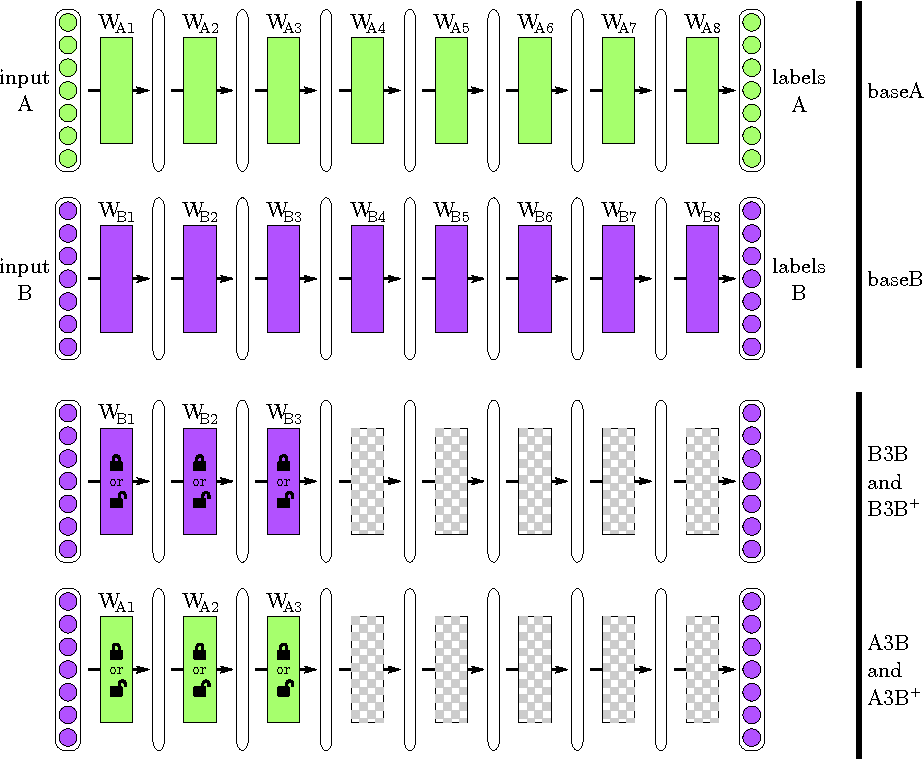
\includegraphics[width=\linewidth]{Chapters/2.Background/figures/transfer_experiment.png}
    \caption[Transfer learning experiment]{Illustration provided by Yosinski et al. in their paper\cite{yosinski2014transferable} in figure 1 to visualize their experimental process. The top two models, A (green) and B (purple), are trained first on data A, then on data B. The labeled rectangles represents each layer in the networks, i.e., \(W_{A_{1}}\) is the weights in layer 1 in model A, and the ellipsoids between each layer represents activation layers. The color of the stack of circles to the left of each model shows which partition of the dataset each model is trained on. The bottom two rows show the first three layers from A and B being transferred to new randomly initialized models. \cite{yosinski2014transferable} showed better accuracy in model A3B than every other model in this figure, even B3B.}
    \label{fig:transferexperiment}
\end{figure}

In a study by Yosinski et al. \cite{yosinski2014transferable}, results showed transferability in the first layers of an image classifier. The experiment proposed using transfer performance as a measure of generality and specificity. The study divided the dataset\footnote{The study used the ImageNet dataset of 2012 which contained 1,281,167 labeled training images and 50,000 test images, each labeled with one of 1000 classes.} randomly in two subsets (A and B), and trained two identical models on each of the subsets. The first \(n\) layers in two randomly initialized models were replaced by the first trained layers from A and B. 

An additional training step, consisting of finetuning the first layers by allowing backpropagation through them, was done on data from subset B. The visualization of this in figure \ref{fig:transferexperiment} is for a case with \(n=3\). The goal was to study the effects transfer had on accuracy when transferring layers from one classification case to another. 

The best results were achieved when training a model on subset A, transferring the first three layers to a new randomly initialized model and fine-tuning these transferred layers while the new model was trained on data-subset B. This confirmed their expectation that the earlier layers in an image classifier get highly generalized and learn to approximate Gabor-filters. In section \ref{exp1:results.quinary} we see tendencies of this behavior. 

\subsection{Multi-task Learning}
Multi-task Learning and Transfer Learning both have the same ideology of sharing some parameter state between tasks to positively influence learning. Where Transfer Learning does not concern itself with performance on a seed task, multi-task learning tries to optimize parameters for multiple tasks. The most common ways of achieving this are by \textit{soft parameter sharing} and \textit{hard parameter sharing}. While both techniques have some weights unique to each task, \textit{hard parameter sharing} optimize the same parameters for all tasks. This is shown to reduce overfitting\cite{hardparametersharing} significantly. As the weights change values to optimize for a changing target, they never overly adapt to the training set. \textit{Soft parameter sharing} on the other hand have separate parameters for each task, but lateral connections between each tasks layers to minimize the distance between the parameters trained for each task.

\subsection{Curriculum Learning}
Both humans and animals learn better when examples provided are ordered and gradually increasing in difficulty. With this motivation, curriculum learning is introduced as a strategy for optimizing the learning process. This technique is shown to increase generalization to data\cite{curriculumlearning} and is the motivation for task ordering in the selection pressure experiments (see \ref{exp2:datasets}).

\section{Catastrophic Forgetting}
\label{background:catastrophicforgetting}
A problem that arises in systems where parameters are trained on multiple sequential tasks is what is called \textit{catastrophic forgetting}. Set in a transfer learning scenario, this effect manifests itself as moving parameters away from an area of low error for a previously trained task. This movement could, for instance, be because the parameters are fine-tuned for a new task. While the performance for the second task increase, performance for the first task decrease because the \textit{knowledge is forgotten} when the weights are re-adapted to the new data. This is not a problem in a scenario where the source task is considered a stepping stone to reach good performance for the target task, but might be if all tasks trained on are of the same importance.

\iffalse
\begin{figure}[ht]
    \centering
    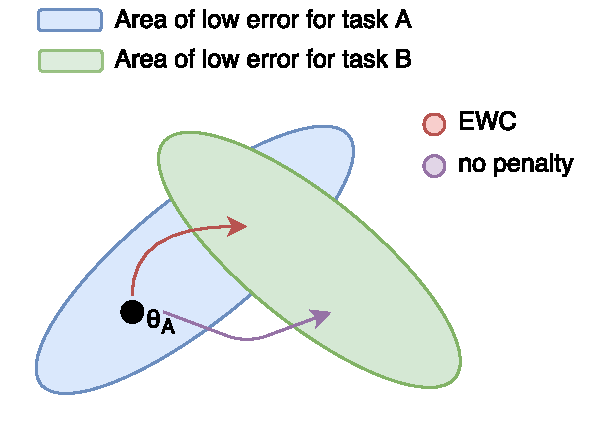
\includegraphics[width=0.7\linewidth]{Chapters/2.Background/figures/EWC.pdf}
    \caption[Elastic Weight Consolidation]{Reconstruction of a figure from the paper on Elastic Weight Consolidation\cite{ewc}. The figure shows the parameter space \(\mathcal{P}\) and hypothetical areas of low error for two tasks A and B. The arrows indicate the direction EWC \textit{red} and normal training \textit{purple} takes the parameters.}
    \label{fig:ewc}
\end{figure}
\subsection{Elastic Weight Consolidation}
Elastic Weight Consolidation (EWC) is a novel algorithm proposed in January of 2017 by Kirkpatrick et al.\cite{ewc}. During the transfer of weights from task A to task B, over-parameterization\footnote{Overestimating the amount of capacity a network need to solve a task.} makes it likely that a solution to problem B lays close to the solution for task A in the parameter space \(\mathcal{P}\)\footnote{A solution may be viewed as a set of parameters \(\bar{\theta}\). For multiple parameters in \(\bar{\theta}_{A}\) as a solution to task A, many configurations of those will give the same performance for the NN and all those sets of \(\bar{\theta}_{A}\) would be considered optimal sets.}. During optimization of parameters \(\bar{\theta}_{B}\) for task B, EWC makes sure the parameters stay within an area of low error for task A as seen in figure \ref{fig:ewc}

Using EWC, Kirkpatrick et al.\cite{ewc} was able to train the same NN on ten different Atari games without the effects of catastrophic forgetting between training tasks. With a human-normalized score of 1 for each game, giving a total possible score\footnote{where is 0 the same as a random agent, and 10 is at least human-level performance on all games.} of 10, the EWC driven training reached a score of around six after 500 million training frames. The control never reached anything higher than 1 as each new task cause parameters to move away from areas of low error for the previous tasks.
\fi

\subsection{Progressive Neural Networks}
Rusu et al. published a paper in September of 2016\cite{progressiveneuralnetworks} where they addressed the problem of catastrophic forgetting during transfer learning with fine-tuning. Their proposed solution, Progressive Neural Networks (PNN), were shown to be able to learn multiple tasks sequentially without overwriting the previously trained weights. This was done by horizontally scaling the DNN with a new stack of layers for each new task.
\begin{figure}[ht]
    \centering
    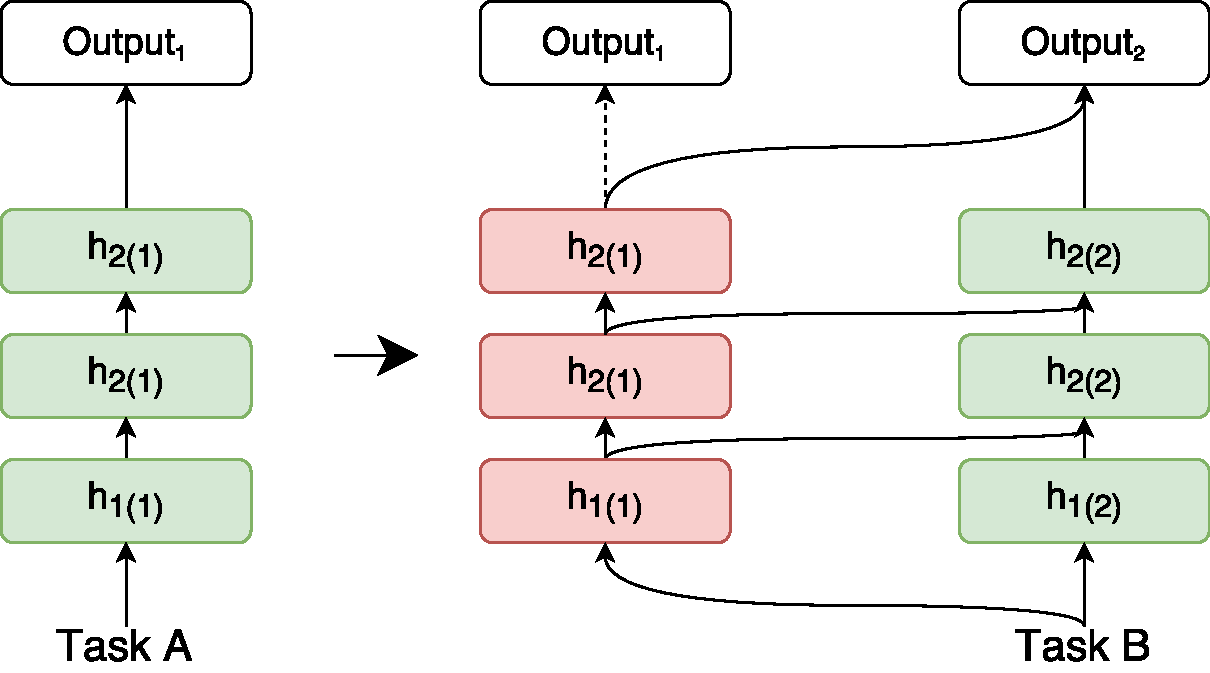
\includegraphics[width=0.8\textwidth]{Chapters/2.Background/figures/ProgressiveNeuralNet.pdf}
    \caption[Progressive Neural Network]{Example of a PNN. \textit{Left}: a three-layer NN is trained on task A. \textit{Right}: Adding another stack of three hidden layers that are being trained on task B. The weights in the first stack trained on A is now locked to the backpropagation from task B, but its weights may still be used (shown by arrows between the layers). Green indicates layer is open to backpropagation, red indicates it is locked. Note that injection of a layer from an older task is not possible as lateral connections are only \textit{to} the new layer. The figure is a simplification of multiple figures from the article\cite{progressiveneuralnetworks}.}
    \label{fig:pnn}
\end{figure}
After training a DNN on a task A\footnote{In the paper, the PNN was used in a RL scenario.}, a new DNN was initialized with lateral connections (see figure \ref{fig:pnn}) to the NN trained on task A and then trained on task B with backpropagation only done through the newly initialized layers. This ensures that the new DNN can optimize freely on task B, but will be able to utilize the weights trained on task A, without catastrophic forgetting occurring in the first DNN. When a sufficient performance on task B is reached, the PNN can perform optimally on both tasks, given some selection of the output (i.e., if given data for a task within the domain A, the output from the weights trained on task B is not optimal). Multiple tasks can be trained using this method. For each new task, a new DNN is initialized, and the other DNNs in the PNN is connected laterally to each new layer. 

We can compare the way each new task is learned to a transfer learning scenario where backpropagation not allowed in the transferred layers (see figure \ref{fig:transferexperiment}). The difference being the layer outputs are calculated in parallel for the two models, and multiple of these outputs may be introduced in the new model through what the paper calls \textit{adapters} (not visualized in \ref{fig:transferexperiment}). These \textit{adapters} performs dimensionality reduction as well as providing tunable scalars so the model can scale lateral connections as needed for the new task.

A problem with this scaling addressed in the paper is that of quadratic growth of parameters for each new training task. Experiments show that there is a reduction in the new capacity utilized by the PNN for each new task added. This implies the growth of the PNN for each new task could decrease exponentially\footnote{Here the paper suggests pruning or online compression during learning.} without needing the new task to follow the same downward trend in complexity. 

\section{Genetic Algorithms}
\label{background:GA}
Genetic Algorithms\cite{GAbook} (GA), a sub-category of evolutionary algorithms,  are biologically inspired algorithms that generate high-quality solutions to optimization and search problems. By mimicking natural operators like \textit{crossover} and \textit{mutation}, GAs views its possible solutions as individual genomes in a population and applies these natural operators on the population in a simplification of how evolution works. 

A vital driving force of GAs is the fitness-function, which maps a genome to a fitness value that can be used to rank solutions (genotypes) by how well they perform. In a real-world example of the fitness function, a \textit{strong} animal of some sort, able to acquire nourishment and fend off potential predators, is given a higher fitness value than a similar animal not as well suited for its environment. The famous term \textit{survival of the fittest} is valid in both this example and the \textit{in silico} representation of evolution. The strongest animal has a higher probability to survive and reproduce, and GAs are implemented to favor solutions that yield high fitness values.  
When a population is ranked by its fitness, different selection schemes can be applied to simulate the natural selection of strongest genomes. This selection function has a direct influence on how diverse the population is in its solutions. While we intuitively would like to remove poor solutions and keep the strong, this might guide the population only to sustain one genotype, at which point we say the population has \textit{converged}. This causes the search to get stuck in a \textit{local optima}, where the space of possible solutions have not been explored thoroughly, and we are not able to say the solution we found is among the best. Instead, the selection function varies which genomes are removed, where the more fit genotypes typically have the highest probability of survival. 

A commonly used way of ordering and discussing genetic algorithms is by the properties \textit{exploration} and \textit{exploitation}. A search with high exploration tries to keep a diverse population where many possible solution types are evaluated to find an area in solution space with high fitness. On the other hand, algorithms with high exploitation will usually find the locally best solution. A way of achieving this is by keeping a uniform population with only small differences in the genomes.

Another property of a genetic search is its \textit{selection pressure}, which describes how much a generations best solution is favored. Having a high selection pressure translates to the best solution having a strong influence on the total population in the next generation, while a minimum selection pressure would cause the search to ignore fitness-rank and arbitrarily select genomes for survival or recombination.

Some recombination of genomes is usually performed with a \textit{crossover} algorithm to keep the population size from shrinking in each generation.  The crossover function takes a set of \textit{parent} genomes and outputs a set of offspring with the goal of controlling the population size.  Typically, a child genome is then mutated under some probability to further maintain genetic diversity. This mutation applies some small genome change.

\begin{figure}[ht]
    \centering
    \begin{subfigure}[ht]{0.25\linewidth}
        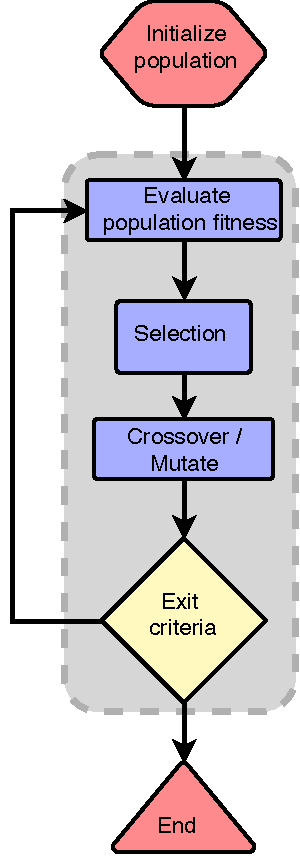
\includegraphics[width=\linewidth]{Chapters/2.Background/figures/GA.pdf}
        %\caption{Genetic Algorithm}
    \end{subfigure}
    \hspace{0.25\textwidth}
    \begin{subfigure}[ht]{0.25\linewidth}
        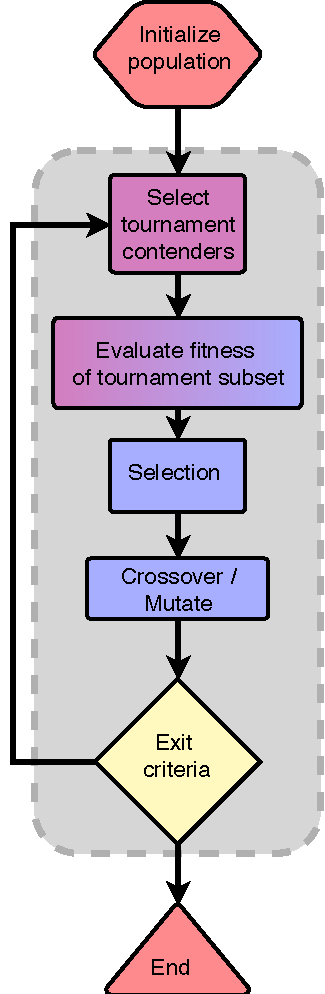
\includegraphics[width=\linewidth]{Chapters/2.Background/figures/TS.pdf}
        %\caption{Tournament Search}
    \end{subfigure}
    \caption[Algorithm flowcharts]{Flowcharts of the general Genetic Algorithm (left) and Tournament Search (right). The color blue indicates the operation is standard in a GA, while purple is special to a tournament search. One complete run of all operations in the gray area constitute one generation.}
    \label{fig:algorithmflowcharts}
\end{figure}

\subsection{Tournament search}
One implementation of a genetic algorithm is the \textit{Tournament Search}. True to the name, in every generation, a subset of the population is selected as contenders in a tournament. The genotypes are evaluated with a fitness function, and some selection scheme chooses genomes to be reinserted back into the population based on the fitness ranking. The selection probability is given as 
\begin{equation}
    \label{eq:tournamentsearch}
    P_{i} = p(1-p)^{i-1}
\end{equation}
where \(i\) is the fitness-ranking achieved during the tournament (1 being first place and so on) and \(p\) is the probability of selecting the first place as survivor. Figure \ref{fig:algorithmflowcharts} juxtapose flowcharts for a general GA and the Tournament Search algorithm. 

In the search implementation used in the experiments in this thesis (see \ref{exp1:implementation}, \ref{exp2:implementation}, and \ref{exp3:implementation}), a version of the tournament search is used. For every generation, a subset of the total population, given by the tournament size, is selected and evaluated. The winner then replaces each of the other contestants, making this selection implementation what is called a \textit{Deterministic Tournament Selection}, e.g., \(p=1\). Before the winner and its duplicate(s) are inserted back into the population, each copy of the winner is mutated under some probability to keep the diversity. 

A benefit of the tournament search, except for its efficiency in implementing and ability to work in parallel architectures, is that the \textit{selection pressure} of the search can easily be adjusted(see \ref{exp2:description}). By increasing the tournament size, the winning genome is replicated more, and future generations are more heavily influenced by that genome. This increased "importance" in being selected as the winner of a tournament is what is described as a \textit{selection pressure}.

\subsection{Population Diversity}
\label{background:diversity}
Population diversity is a metric assigned to a population that describes its internal difference between genomes and is mentioned here because of its importance to the experiments in chapter \ref{exp2} and \ref{exp3}. This diversity value translates to how efficiently a search explores the solution space, as the more similar the genomes in a population is, the more restricted is the coverage of the search space. The goal of this metric is to provide a scalar value corresponding to the spread of genomes in genotypic space. 

Take for instance two binary genomes a and b as a population.
\begin{equation*}
    \begin{split}
        a = [0, 1, 1, 0, 0, 1, 1]\\
        b = [0, 0, 0, 1, 0, 1, 0]\\
        F_{\text{Diversity}}(a, b)=d_{1}
    \end{split}
\end{equation*}
The diversity function \(F_{\text{Diversity}}(a, b)\) gives a scalar value \(d_{1}\). If we change the genome \(b\) to something more like \(a\), the new diversity \(d_{2}\) is smaller than \(d_{1}\) as the total diversity in the population has been reduced. 

\subsubsection{Pair-wise Hamming Distance}
One of the most commonly used measures of distance in genotypic space\cite{populationDiversity} is the pair-wise Hamming distance given by the equation 
\begin{equation}
    \label{eq:Hamming}
    H=\sum_{j=1}^{j=P-1}\sum_{{j}'=j+1}^{{j}'=P}\sum_{i=1}^{i=L}\left |y_{ij}-y_{i{j}'}\right |
\end{equation}
where P is the population size, L is the length of genomes and \(y_{ji}\) is the i-th gene in genome j. In experiments in chapter \ref{exp2} and \ref{exp3}, a reduced form of this formula is used to calculate diversity (see appendix \ref{appendix:Hammingreduction} for reduction proof). While Hamming distance provides a good metric for diversity, some cases can cause Hamming distance to misrepresent a change in diversity. 

Take, for instance, the populations 
\begin{equation*}
    \begin{split}
        [0, 0, 1, 1]\\
        [1, 1, 0, 0]\\
        [1, 0, 0, 1]\\
    \end{split}
\end{equation*}
which have 3 separate genotypes and a Hamming distance of 8. Reducing the diversity in this population by setting the third genome to be equal to the second, changes the population to 
\begin{equation*}
    \begin{split}
        [0, 0, 1, 1]\\
        [1, 1, 0, 0]\\
        [1, 1, 0, 0]\\
    \end{split}
\end{equation*}
The diversity in this population have obviously dropped, but the Hamming distance is still 8, making the Hamming metric misrepresenting the diversity when duplicates of genomes appear in a population. 

\subsubsection{Frequency Diversity}
In some cases where a population contains duplicated genomes, counting the number of unique genomes can provide a more accurate diversity metric than pair-wise Hamming distance. However, the \textit{frequency of unique genomes} is quite poor as a diversity metric by itself, as there is no nuance to the similarity. I.e., for a population of two identical genomes, changing one gene in one of the genomes would increase the diversity by the same amount as changing all genes. 

In the experiments in chapter \ref{exp2} and \ref{exp3}, both frequency diversity and Hamming distance are used to create a full picture of how the diversity changes during a search.

\section{PathNet}
\label{background:pn}
In 2017, DeepMind took the modular approach\footnote{Modular with respect to the traditional approaches of transfer from monolithic models.} to deep transfer learning for multi-task systems one step further with their newly developed Super Neural Network structure\footnote{A Super Neural Network is a meta-network where each node in the network is itself a Neural Network.}; \textit{PathNet}\cite{pathnet}. Where Progressive Neural Networks transfer knowledge between domains by adding a new uninitialized DNN for each task, the size of PathNet is not dynamic in the number of parameters. At training start, the net consists of randomly initialized weights in multiple DNNs, where each DNN is considered a module (or node) in a larger PathNet structure. 

Using a combination of evolutionary and machine learning techniques, PathNet shares the PNNs traits of being able to optimize for multiple training tasks without catastrophic forgetting and transfer knowledge between tasks by reusing weights locked to backpropagation.  
\begin{figure}[ht]
    \centering
    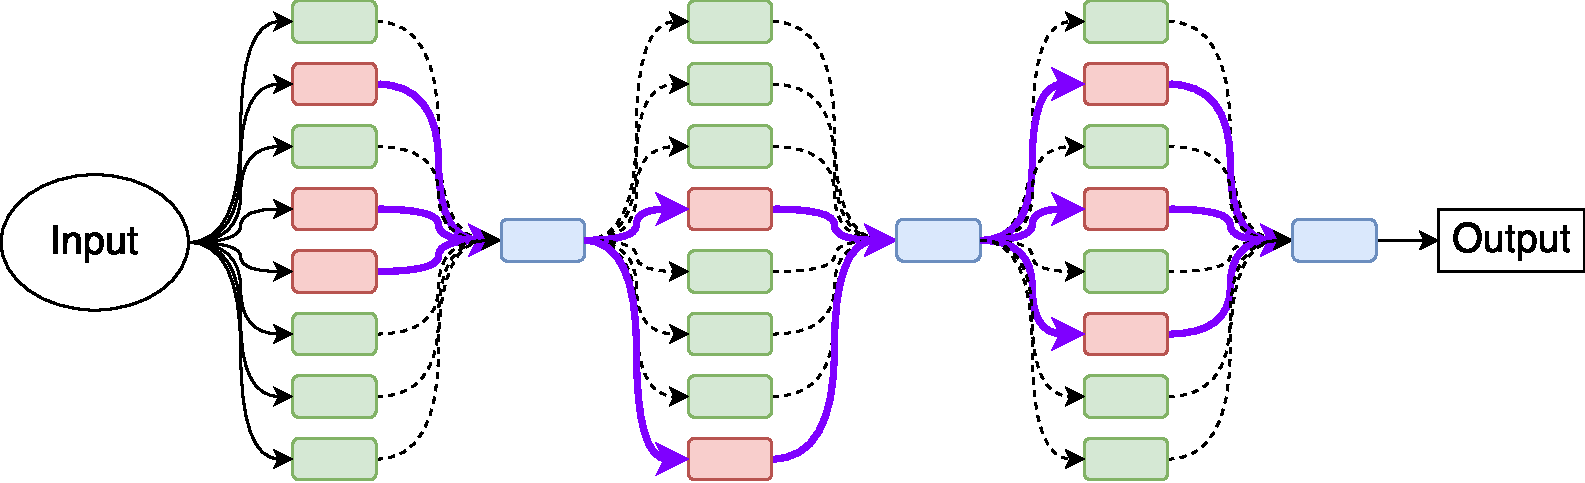
\includegraphics[width=0.8\textwidth]{Chapters/2.Background/figures/PathNet.pdf}
    \caption[PathNet structure]{The Figure shows a PathNet implementation with 3 layers of 8 modules (NNs) in each layer. The \textit{red} color indicates that the weights of this NN are locked to backpropagation, while \textit{green} indicates it is open. \textit{Blue} cells are reduced-sum modules which summarize the features between each layer. The purple connections show a path through the network. One path may use multiple modules from each layer and may contain both locked and open modules.}
    \label{fig:pathnet}
\end{figure}

\subsection{Structure}
The PathNet consists of layers of modules, where each layer has a set number of modules as seen in figure \ref{fig:pathnet}. Each module is in itself a neural network of some sort, where the type of NN is adapted to the relevant task. Between each layer, the output from each active module is passed through a reduced-sum operator that adds together each output element-wise to keep the dimensionality of the output from scaling by the number of active modules. 

Each task applied to PathNet is designated a unique end-layer added to every path created for that task, meaning all paths in a search has the same final layer specific to that task. This layer defines the output and activation function that fit the problem at hand, be it a classification task, regression or something else.  

A \textit{path} is the name given a subset of the modules in a PathNet structure, where the path may contain between 1 and \(\omega\) modules from each layer, where \(\omega\) is adjusted to control the amount of capacity (number of weights) allocated to a path (solution). Each module in this path is locked after training is completed. This locking of the modules is to prevent the weights in the modules from changing if they are reused by subsequent tasks, and this preventative measure is what ensures that catastrophic forgetting does not occur in this structure. After the optimal path is found, the rest of the modules that are not currently used and does not contain optimized weights for any task is reinitialized. Fernando et al. claims\cite{pathnet} that this re-initialization is because they were not able to reach results that outperformed fine-tuning without it.

\subsection{Search}\label{background:pathnet.search}
For every new task introduced to the PathNet, a tournament search algorithm is initialized to find an optimal path through the network. A population of pathways (e.g., subsets of modules) are randomly initialized and subjected to a tournament search with a tournament size of 2 and probability \(p=1\) of selecting the winner (as per equation \ref{eq:tournamentsearch}), making this tournament implementation deterministic. Every fitness evaluation of the tournament contenders is done by training them each a set amount and using the negative loss as a fitness value. One \textit{training unit} is quite small at 50 batches\footnote{The loss-value is usually calculated for \textit{batches} of data at the same time to average out potential outliers in the training data.} of 16 examples each. This means that evaluating the fitness of a path changes the performance of that path unless all modules in that path are locked to backpropagation.

When a winner is selected, the genome of the winner is duplicated to replace the looser and then mutated. Each module used in the path have the probability \(\frac{1}{L\omega}\) of being replaced with a neighboring module\footnote{A module with index \(i\) is replaced with a module of index between \(i-2\) and \(i+2\)}, where L is the number of layers, and \(\omega\) is as mentioned the max number of active modules in each layer. The mutation ensures that the average path experience a genome change that separates it from the winner. Over multiple generations however, the population converges to a lower diversity state where more and more paths contain similar modules. The search is terminated under some criteria, either a reached threshold fitness or a generation limit. 

If an optimal path found for a task contain a module that was trained during a search for a different task, the newly trained path have \textit{one unit of module reuse}. This metric is an important measure for the experiments in chapter \ref{exp1}, \ref{exp2}, and \ref{exp3}.

\section{Statistical methods}
\subsection{Monte-Carlo probability estimation}
\label{mc-estimate}
Given the nature of the systems used in this thesis, analytically calculating the probability of certain outcomes\footnote{In experiments \ref{exp1} and \ref{exp2}, the amount of module reuse for a random path selection is used as a comparison to experimental outcomes.} is quite hard. In such cases, the probability of certain outcomes can be estimated with a Monte-Carlo approach. This is done by simulating some scenario governed by some stochastic properties for \(n\) number of trials and measuring some \(N\) number of outcomes. The probability \(p\) of these outcomes occurring can be estimated as 
\begin{equation*}
    \hat{p}=\frac{N}{n}
\end{equation*}
Since the error here is non-biased random with a mean error of zero, the standard deviation can be given as the square root of the mean squared error 
\begin{equation*}
    \sigma=\sqrt{E[(\hat{p}-p)^{2}]} =\sqrt{\frac{p(1-p)}{n}}
\end{equation*}


Selecting a sufficiently large \(n\) can be a problem with the Monte-Carlo approach since \(p\) is unknown. Still, we can for a fixed \(n\) select a maximum standard deviation we want and calculate the size of \(p\) at which point we lose accuracy. 

For a maximum ratio between the standard deviation \(\sigma\) and \(p\) of \(R\)\footnote{I.e: \(R=0.01\) means the probability of the measured outcome is 100 times larger than the standard deviation.} and \(n\) being the number of trials, we can calculate maximum of \(p\) as
\begin{equation*}
    \frac{\sqrt{E[(\hat{p}-p)^{2}]}}{p} < R
\end{equation*}
\begin{equation*}
    \frac{1}{p}\sqrt{\frac{p(1-p)}{n}} < R
\end{equation*}
\begin{equation*}
    \frac{1-p}{np} < R^{2}
\end{equation*}
\begin{equation*}
    \frac{1}{p}< nR^{2}+1
\end{equation*}
\begin{equation}
    \frac{1}{nR^{2}+1}<p
    \label{eq:montecarloP}
\end{equation}
This means a Monte-Carlo simulation of \(10^{6}\) trials where we want the error to be within  \(0.01\) of \(p\), lose certainty if the probability is smaller than \(\frac{1}{101}\).

\subsection{Comparing results}
When comparing observations during experimentation, hypothesis-testing is a way of providing gravitas to observational differences. A method is used to test a statement about the data (called a null-hypothesis or \(H_{0}\)) by providing a p-value. This p-value is compared to a predetermined significance level (usually 0.05) and provides a metric that describes the likelihood of the null-hypothesis being valid\footnote{A low p-value corresponds to a low likelihood.}. The assumption being: we can claim an hypotheses to be true if the counter-claim is unlikely.  

\subsubsection{Mann–Whitney–Wilcoxon test}
\label{background:mannwhitney}
When calculating a P-value, the effectiveness of the method used depends highly on the observations tested. In this thesis, we can not assume normality in the data, nor equal variance. Therefore a non-parametric method for comparison is used: Mann-Whitney-Wilcoxon (MWW) testing. This test provides a U-value used to reject or accept the null-hypothesis that two groups of observations have the same distribution. 

The assumptions laying behind the use of MWW are 
\begin{itemize}
    \item Rank-able continuous or ordinal data.
    \item Independent groups.
    \item Independencies in observations between groups.
    \item Whether the two distributions have the same or different shape is known. 
\end{itemize}
These assumptions are determined to be met in the case of these experiments. 

The cases MWW is applied here contains small groups of observations, the direct explanation of how a U-value is calculated is the quickest. 

For two groups of observations, each observation is ranked by its value\footnote{In the case of the experiments in chapter \ref{exp2} and \ref{exp3} the observations are classification validation accuracies, and each trial result is naturally ranked by this accuracy-value.}. The U-value for the group \(i\) is given as 
\begin{equation*}
    U_{i} = R_{i}-\frac{n_{i}(n_{i}+1)}{2}
\end{equation*}
where \(R_{i}\) is the sum of ranks in group \(i\) and \(n_{i}\) is the number of observations in that group. 
Calculating a \(U_{i}\) for each group tested provides two U-values where the smallest one is compared to a critical U value where the null-hypothesis is rejected if 
\begin{equation*}
    min(U_{1}, U_{2}) \leq U_{\text{Critical}}
\end{equation*}

\subsubsection{Bonferroni correction}
As the MWW rank-sum test is not multivariate, multiple tests are performed in sections \ref{exp2} and \ref{exp3} to compare all algorithms. Because the scaling probability that some of the results are unlikely, a Bonferroni correction of the significance level is done to combat the increasing probability of encountering unlikely results. 

The desired significance level is scaled by the inverse of the number of tested hypotheses \(m\). 
\begin{equation*}
    \alpha=\frac{\alpha_{\text{Desired}}}{m}
\end{equation*}
